\documentclass[justified, 11pt]{scrartcl}\usepackage[]{graphicx}\usepackage[]{xcolor}
% maxwidth is the original width if it is less than linewidth
% otherwise use linewidth (to make sure the graphics do not exceed the margin)
\makeatletter
\def\maxwidth{ %
  \ifdim\Gin@nat@width>\linewidth
    \linewidth
  \else
    \Gin@nat@width
  \fi
}
\makeatother

\definecolor{fgcolor}{rgb}{0.345, 0.345, 0.345}
\newcommand{\hlnum}[1]{\textcolor[rgb]{0.686,0.059,0.569}{#1}}%
\newcommand{\hlstr}[1]{\textcolor[rgb]{0.192,0.494,0.8}{#1}}%
\newcommand{\hlcom}[1]{\textcolor[rgb]{0.678,0.584,0.686}{\textit{#1}}}%
\newcommand{\hlopt}[1]{\textcolor[rgb]{0,0,0}{#1}}%
\newcommand{\hlstd}[1]{\textcolor[rgb]{0.345,0.345,0.345}{#1}}%
\newcommand{\hlkwa}[1]{\textcolor[rgb]{0.161,0.373,0.58}{\textbf{#1}}}%
\newcommand{\hlkwb}[1]{\textcolor[rgb]{0.69,0.353,0.396}{#1}}%
\newcommand{\hlkwc}[1]{\textcolor[rgb]{0.333,0.667,0.333}{#1}}%
\newcommand{\hlkwd}[1]{\textcolor[rgb]{0.737,0.353,0.396}{\textbf{#1}}}%
\let\hlipl\hlkwb

\usepackage{framed}
\makeatletter
\newenvironment{kframe}{%
 \def\at@end@of@kframe{}%
 \ifinner\ifhmode%
  \def\at@end@of@kframe{\end{minipage}}%
  \begin{minipage}{\columnwidth}%
 \fi\fi%
 \def\FrameCommand##1{\hskip\@totalleftmargin \hskip-\fboxsep
 \colorbox{shadecolor}{##1}\hskip-\fboxsep
     % There is no \\@totalrightmargin, so:
     \hskip-\linewidth \hskip-\@totalleftmargin \hskip\columnwidth}%
 \MakeFramed {\advance\hsize-\width
   \@totalleftmargin\z@ \linewidth\hsize
   \@setminipage}}%
 {\par\unskip\endMakeFramed%
 \at@end@of@kframe}
\makeatother

\definecolor{shadecolor}{rgb}{.97, .97, .97}
\definecolor{messagecolor}{rgb}{0, 0, 0}
\definecolor{warningcolor}{rgb}{1, 0, 1}
\definecolor{errorcolor}{rgb}{1, 0, 0}
\newenvironment{knitrout}{}{} % an empty environment to be redefined in TeX

\usepackage{alltt}

% template based on Wenneker Assignment - Frits Wenneker template

% packages {
  \usepackage{amsmath, amsfonts, amsthm} 
  \usepackage{listings}
  \usepackage{graphicx}
  \usepackage{booktabs}
  \usepackage{enumitem}
  \usepackage{scrlayer-scrpage}
  \usepackage{sectsty}
  \usepackage{geometry} % Required for adjusting page dimensions and margins
  \usepackage[portuguese]{babel}
  \usepackage{booktabs}
  \usepackage{longtable}
  \usepackage{array}
  \usepackage{multirow}
  \usepackage{wrapfig}
  \usepackage{float}
  \usepackage{colortbl}
  \usepackage{pdflscape}
  \usepackage{tabu}
  \usepackage{threeparttable}
  \usepackage{threeparttablex}
  \usepackage[normalem]{ulem}
  \usepackage{makecell}
  \usepackage{xcolor}
  \usepackage{comment}
  \usepackage{lipsum}
  \usepackage{tabulary}
  \usepackage{tabularx}
  \usepackage{hyperref}
  \usepackage{cite}
  % \usepackage{showframe}
% }


\sectionfont{\vspace{6pt}\centering\normalfont\scshape} % \section{} styling
\subsectionfont{\normalfont\bfseries} % \subsection{} styling
\subsubsectionfont{\normalfont\itshape} % \subsubsection{} styling
\paragraphfont{\normalfont\scshape} % \paragraph{} styling


\ohead*{} % Right header
\ihead*{} % Left header
\chead*{} % Centre header

\ofoot*{} % Right footer
\ifoot*{} % Left footer
\cfoot*{\pagemark} % Centre footer

\setlist{noitemsep}

\geometry{
	paper=a4paper, % Paper size, change to letterpaper for US letter size
	top=2.5cm, % Top margin
	bottom=3cm, % Bottom margin
	left=3cm, % Left margin
	right=3cm, % Right margin
	headheight=0.75cm, % Header height
	footskip=1.5cm, % Space from the bottom margin to the baseline of the footer
	headsep=0.75cm, % Space from the top margin to the baseline of the header
	%showframe, % Uncomment to show how the type block is set on the page
}

\floatplacement{figure}{H}
\floatplacement{table}{H}

\title{	
	\normalfont\normalsize
	\textsc{ISCTE-IUL \\ Licenciatura de Ciência de Dados}\\
	\vspace{25pt} 
	\rule{\linewidth}{0.5pt}\\
	\vspace{20pt}
	{\huge TODO Título}\\ 
  \vspace{12pt} 
  {\large TODO Subtítulo}\\
	\vspace{12pt}
	\rule{\linewidth}{2pt}\\
	\vspace{12pt} 
}
\author{
  André Plancha, 105289 \\
  <Andre\_Plancha@iscte-iul.pt> \\
  Tomás Ribeiro, 105220 \\
  <tfroo1@iscte-iul.pt> \\
  Afonso Silva, 105208 \\
  <agsos@iscte-iul.pt> \\
  Rui Chaves, 104914 \\
  <rfpcs1@iscte-iul.pt>
}
\date{20/12/2022 \\ Versão 0.0.2} % 
\IfFileExists{upquote.sty}{\usepackage{upquote}}{}
\begin{document}
\maketitle


% TODO introducao
\begin{knitrout}
\definecolor{shadecolor}{rgb}{0.969, 0.969, 0.969}\color{fgcolor}\begin{kframe}
\begin{alltt}
\hlstd{df} \hlkwb{<-} \hlkwd{read.csv}\hlstd{(}\hlkwd{here}\hlstd{(}\hlstr{"data"}\hlstd{,} \hlstr{"listings.csv"}\hlstd{))}
\hlstd{shape} \hlkwb{<-} \hlkwd{st_read}\hlstd{(}\hlkwd{here}\hlstd{(}\hlstr{"data"}\hlstd{,} \hlstr{"SF Planning Neighborhood Groups Map"}\hlstd{))}
\hlkwd{tmap_mode}\hlstd{(}\hlstr{"plot"}\hlstd{)}
\hlstd{shape_plot} \hlkwb{<-} \hlstd{shape} \hlopt
    \hlkwd{ggplot}\hlstd{()} \hlopt{+} \hlkwd{geom_sf}\hlstd{()} \hlopt{+} \hlkwd{theme}\hlstd{(}\hlkwc{legend.position} \hlstd{=} \hlstr{"bottom"}\hlstd{)}
\end{alltt}
\end{kframe}
\end{knitrout}

A base de dados que nos foi disponibilizada vem do  projeto, fundado por Murray Cox com a missão de "[...] fornecer dados e defesa sobre o impacto do Airbnb em comunidades residenciais"\cite{InsideAirBnbAbt}.

A base de dados contém 6629 entradas, e cada uma delas representa um registo de um anúncio para o aluguer de um alojamento disponível no Airbnb, em São Francisco, Califórnia. Cada alojamento contém informação sobre o seu preço, localização, hospedeiro, o tipo de alojamento, as \textit{reviews} do alojamento, e licensa do alojamento.

\begin{knitrout}
\definecolor{shadecolor}{rgb}{0.969, 0.969, 0.969}\color{fgcolor}\begin{kframe}
\begin{alltt}
\hlkwd{data.frame}\hlstd{(}\hlkwc{row.names} \hlstd{=} \hlkwd{colnames}\hlstd{(df),} \hlkwc{type} \hlstd{=} \hlkwd{sapply}\hlstd{(df,}
    \hlstd{class))} \hlopt
    \hlkwd{showT}\hlstd{()}
\end{alltt}
\end{kframe}\begin{table}
\centering\begingroup\fontsize{10}{12}\selectfont

\begin{tabular}{l|r}
\hline
  & type\\
\hline
\cellcolor{gray!6}{id} & \cellcolor{gray!6}{numeric}\\
\hline
name & character\\
\hline
\cellcolor{gray!6}{host\_id} & \cellcolor{gray!6}{integer}\\
\hline
host\_name & character\\
\hline
\cellcolor{gray!6}{neighbourhood\_group} & \cellcolor{gray!6}{logical}\\
\hline
neighbourhood & character\\
\hline
\cellcolor{gray!6}{latitude} & \cellcolor{gray!6}{numeric}\\
\hline
longitude & numeric\\
\hline
\cellcolor{gray!6}{room\_type} & \cellcolor{gray!6}{character}\\
\hline
price & integer\\
\hline
\cellcolor{gray!6}{minimum\_nights} & \cellcolor{gray!6}{integer}\\
\hline
number\_of\_reviews & integer\\
\hline
\cellcolor{gray!6}{last\_review} & \cellcolor{gray!6}{character}\\
\hline
reviews\_per\_month & numeric\\
\hline
\cellcolor{gray!6}{calculated\_host\_listings\_count} & \cellcolor{gray!6}{integer}\\
\hline
availability\_365 & integer\\
\hline
\cellcolor{gray!6}{number\_of\_reviews\_ltm} & \cellcolor{gray!6}{integer}\\
\hline
license & character\\
\hline
\end{tabular}
\endgroup{}
\end{table}

\end{knitrout}
De forma a perceber melhor a base dados, o \textit{Airbnb} disponibiliza de um "dicionário de dados"\cite{DicDadosAirBnb} que explica o significado de cada uma das variáveis:

\begin{itemize}
  \item \textbf{id}: Número que representa um identificador único do anúncio;
  \item \textbf{name}: Título do anúncio;
  \item \textbf{host\_id}: Identificador único da conta do hospedeiro;
  \item \textbf{host\_name}: Nome da conta do hospedeiro (Normalmente este campo inclui apenas o primeiro nome ou nome da instituição hospedeira);
  \item \textbf{neighbourhood\_group}: Este campo encontra-se vazio e não inclui descrição no dicionário;
  \item \textbf{neighbourhood}: Embora este campo não inclua descrição no dicionário, nesta base de dados este campo representa os bairros de São Francisco como definido pelo Departamento de Planeamento da cidade (os bairros de São Francisco não contém fronteiras oficiais e dependem da fonte (\url{tldrify.com/19p8}), logo a definição das fronteiras definidas pelo Airbnb tiveram de ser determinadas; mais à frente será demonstrado as fronteiras);
  \item \textbf{latitude/longitude}: Coordenadas geográficas do alojamento;
  \item \textbf{room\_type}: Tipo de alojamento, entre "Quarto privado", "Quarto partilhado", "Quarto de hotel", e "Casa/Apartamento inteiro";
  \item \textbf{price}: Preço do alojamento por noite em USD;
  \item \textbf{minimum\_nights}: Número mínimo de noites que o hospedeiro exige para alugar o alojamento;
  \item \textbf{number\_of\_reviews}: Número total de \textit{reviews} que o alojamento tem desde o seu registo no Airbnb;
  \item \textbf{last\_review}: Data da última \textit{review} que o alojamento recebeu;
  \item \textbf{reviews\_per\_month}: Número médio de \textit{reviews} que o alojamento recebe por mês;
  \item \textbf{calculated\_host\_listings\_count}: Número de alojamentos que o hospedeiro tem disponíveis em São Francisco;
  \item \textbf{availability\_365}: Número de dias que o alojamento está disponível por ano.
  \item \textbf{number\_of\_reviews\_ltm}: Número de \textit{reviews} que o alojamento recebeu nos últimos 12 meses;
  \item \textbf{license}: A licença/autorização/número de registo do alojamento.
\end{itemize}

Para o nosso objetivo, algumas colunas não vão ser úteis, devido à sua naturaza. Estas são o id, name, as categorias que referem informações sobre o hóspede (estas colunas conseguem justificar valores atípicos, principalmente em termos de preço; e.g. Um preço extremamente alto pode acontecer devido a um hotel de luxo na cidade. Estes problemas vão ser discutidos mais à frente.), a disponibilidade do alojamento durante o ano, e a licença do alojamento. Como o nosso objetivo será prever o preço esperado baseado na localização do apartamento, não vamos também utilizar variáveis associadas aos hóspedes, como o número de \textit{reviews} e o número de alojamentos que o hóspede tem disponíveis em São Francisco. 
Cada registo contém as coordenadas geográficas e se as representármos graficamente, podemos verificar que grande parte dos alojamentos se encontram concentrados a nordeste da cidade, principalmente em \textit{Downtown/Civic Center}. Apesar disso, também existem muitos alojamentos no resto da cidade.
\begin{knitrout}
\definecolor{shadecolor}{rgb}{0.969, 0.969, 0.969}\color{fgcolor}\begin{kframe}
\begin{alltt}
\hlstd{shape_plot} \hlopt{+} \hlkwd{geom_point}\hlstd{(}\hlkwc{data} \hlstd{= df,} \hlkwd{aes}\hlstd{(}\hlkwc{y} \hlstd{= latitude,}
    \hlkwc{x} \hlstd{= longitude),} \hlkwc{alpha} \hlstd{=} \hlnum{0.5}\hlstd{,} \hlkwc{color} \hlstd{=} \hlstr{"red"}\hlstd{,}
    \hlkwc{size} \hlstd{=} \hlnum{0.1}\hlstd{)}
\end{alltt}
\end{kframe}\begin{figure}
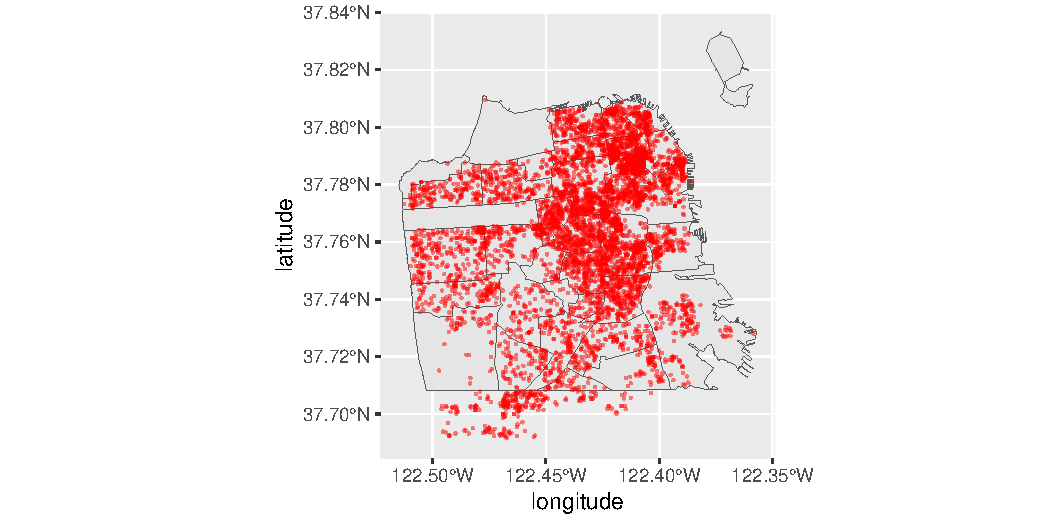
\includegraphics[width=\maxwidth]{figure/chunk-plotPlace-1} \end{figure}

\end{knitrout}
Inesperadamente, o mapa mostra alguns pontos de alojamento fora da cidade, mas julgamos que não vá interferir com as nossas análises, devido ao correto agrupamento (demonstrado mais à frente) e à proximidade da cidade. Embora a razão nos seja desconhecida, acreditamos que o próprio Airbnb agrupa desta forma esses locais devido à sua proximidade com a cidade. \\
A concentração torna-se mais óbvia quando visualizamos o mapa de calor.
\begin{knitrout}
\definecolor{shadecolor}{rgb}{0.969, 0.969, 0.969}\color{fgcolor}\begin{kframe}
\begin{alltt}
\hlstd{rast} \hlkwb{<-} \hlstd{(shape_plot} \hlopt{+} \hlkwd{stat_bin2d}\hlstd{(}\hlkwc{data} \hlstd{= df,}
    \hlkwd{aes}\hlstd{(}\hlkwc{x} \hlstd{= longitude,} \hlkwc{y} \hlstd{= latitude),} \hlkwc{alpha} \hlstd{=} \hlnum{0.7}\hlstd{,}
    \hlkwc{bins} \hlstd{=} \hlnum{30}\hlstd{,} \hlkwc{linejoin} \hlstd{=} \hlstr{"round"}\hlstd{)} \hlopt{+} \hlkwd{scale_fill_viridis_c}\hlstd{(}\hlkwc{option} \hlstd{=} \hlstr{"C"}\hlstd{))}
\hlstd{rast}
\end{alltt}
\end{kframe}\begin{figure}
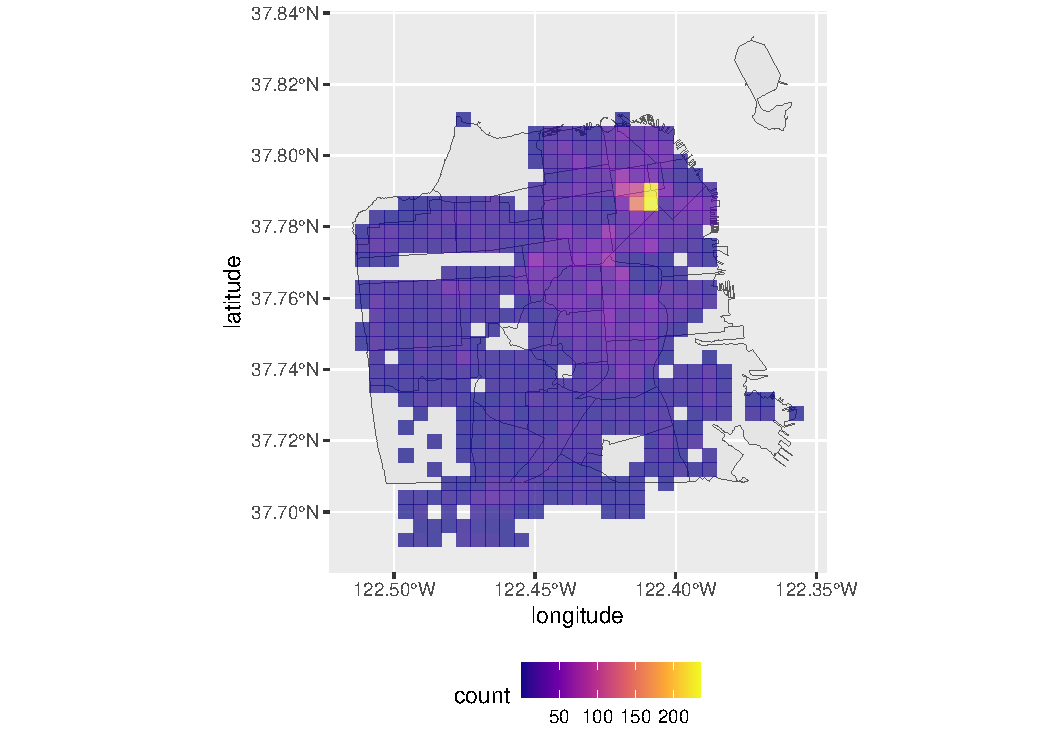
\includegraphics[width=\maxwidth]{figure/chunk-rasterPlaces-1} \end{figure}

\end{knitrout}
O mapa claramente demonstra a concentração de alojamentos na zona clara, mas também consegue-se observar uma grande quantidade, embora mais dispersos, na zona central. Este gráfico demonstra uma possibilidade de agrupar os alojamentos nestas zonas.
\begin{knitrout}
\definecolor{shadecolor}{rgb}{0.969, 0.969, 0.969}\color{fgcolor}\begin{kframe}
\begin{alltt}
\hlstd{df} \hlopt
    \hlkwd{group_by}\hlstd{(neighbourhood)} \hlopt
    \hlkwd{summarise}\hlstd{(}\hlkwc{n} \hlstd{=} \hlkwd{n}\hlstd{(),} \hlkwc{freq} \hlstd{= n}\hlopt{/}\hlkwd{nrow}\hlstd{(df))} \hlopt
    \hlkwd{arrange}\hlstd{(}\hlopt{-}\hlstd{n)} \hlopt
    \hlkwd{head}\hlstd{(}\hlnum{8}\hlstd{)} \hlopt
    \hlkwd{showT}\hlstd{()}
\end{alltt}
\end{kframe}\begin{table}
\centering\begingroup\fontsize{10}{12}\selectfont

\begin{tabular}{r|r|r}
\hline
neighbourhood & n & freq\\
\hline
\cellcolor{gray!6}{Downtown/Civic Center} & \cellcolor{gray!6}{745} & \cellcolor{gray!6}{0.1123850}\\
\hline
Mission & 558 & 0.0841756\\
\hline
\cellcolor{gray!6}{South of Market} & \cellcolor{gray!6}{450} & \cellcolor{gray!6}{0.0678835}\\
\hline
Western Addition & 418 & 0.0630563\\
\hline
\cellcolor{gray!6}{Nob Hill} & \cellcolor{gray!6}{328} & \cellcolor{gray!6}{0.0494796}\\
\hline
Outer Sunset & 281 & 0.0423895\\
\hline
\cellcolor{gray!6}{Bernal Heights} & \cellcolor{gray!6}{280} & \cellcolor{gray!6}{0.0422386}\\
\hline
Haight Ashbury & 276 & 0.0416352\\
\hline
\end{tabular}
\endgroup{}
\end{table}

\end{knitrout}
A tabela mostra que grande parte dos alojamentos listados estão localizados no distrito de \textit{Downtown/Civic Center} e \textit{Mission}.

\begin{knitrout}
\definecolor{shadecolor}{rgb}{0.969, 0.969, 0.969}\color{fgcolor}\begin{kframe}
\begin{alltt}
\hlstd{shape_plot} \hlopt{+} \hlkwd{geom_point}\hlstd{(}\hlkwc{data} \hlstd{= df,} \hlkwd{aes}\hlstd{(}\hlkwc{y} \hlstd{= latitude,}
    \hlkwc{x} \hlstd{= longitude,} \hlkwc{color} \hlstd{= neighbourhood),}
    \hlkwc{alpha} \hlstd{=} \hlnum{0.5}\hlstd{,} \hlkwc{size} \hlstd{=} \hlnum{0.1}\hlstd{)} \hlopt{+} \hlkwd{geom_point}\hlstd{(}\hlkwc{data} \hlstd{= (df} \hlopt
    \hlkwd{filter}\hlstd{(neighbourhood} \hlopt{==} \hlstr{"Downtown/Civic Center"}\hlstd{)),}
    \hlkwd{aes}\hlstd{(}\hlkwc{y} \hlstd{= latitude,} \hlkwc{x} \hlstd{= longitude),} \hlkwc{color} \hlstd{=} \hlstr{"red"}\hlstd{,}
    \hlkwc{alpha} \hlstd{=} \hlnum{1}\hlstd{,} \hlkwc{size} \hlstd{=} \hlnum{0.1}\hlstd{)} \hlopt{+} \hlkwd{theme}\hlstd{(}\hlkwc{legend.position} \hlstd{=} \hlstr{"none"}\hlstd{)}
\end{alltt}
\end{kframe}\begin{figure}
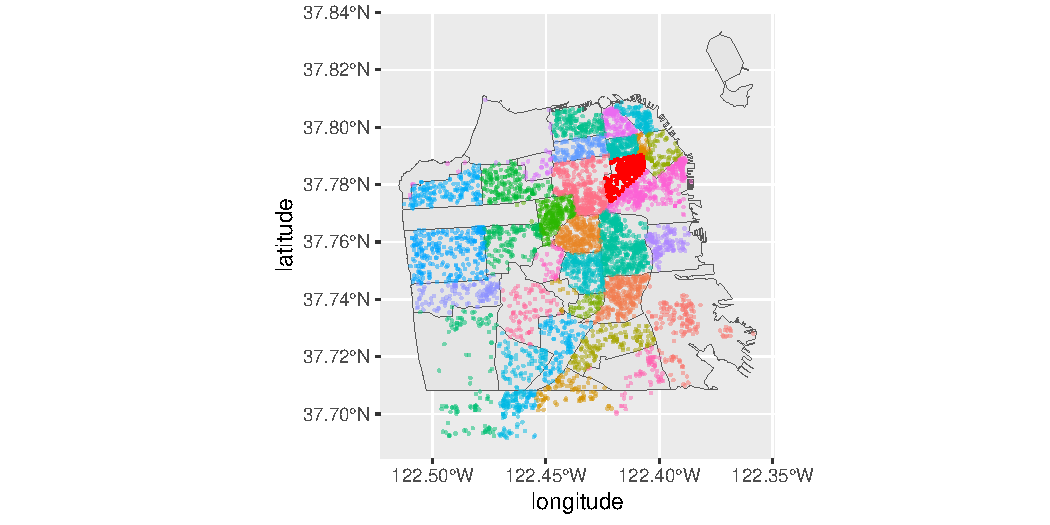
\includegraphics[width=\maxwidth]{figure/chunk-plotNeighbs-1} \end{figure}

\end{knitrout}
Esta figura demonstra que os bairros estão em conformidade com a definição do Departamento de Planejamento da cidade. Mostra também a posição do distrito \textit{Downtown/Civic Center} a vermelho, através do mapa de calor.

\begin{knitrout}
\definecolor{shadecolor}{rgb}{0.969, 0.969, 0.969}\color{fgcolor}\begin{kframe}
\begin{alltt}
\hlkwd{ggplot}\hlstd{(}\hlkwc{data} \hlstd{= df,} \hlkwd{aes}\hlstd{(price))} \hlopt{+} \hlkwd{geom_boxplot}\hlstd{()} \hlopt{+}
    \hlkwd{coord_flip}\hlstd{()}
\end{alltt}
\end{kframe}\begin{figure}
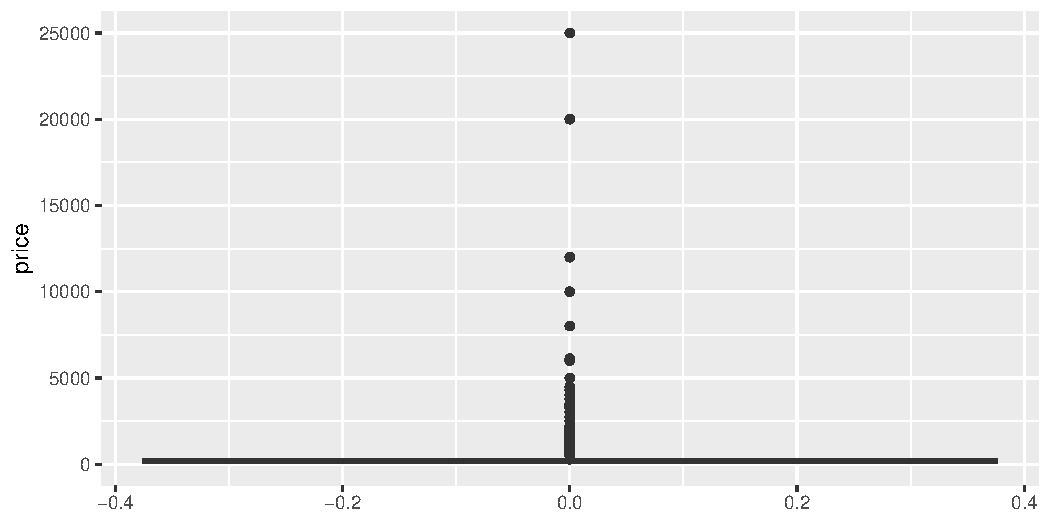
\includegraphics[width=\maxwidth]{figure/chunk-priceBoxPlot-1} \end{figure}

\end{knitrout}
Neste \textit{boxplot} do preço conseguimos notar imediatamente a existência de muitos valores atípicos, que equivalem a preços muito altos tendo em conta a média de preços dos registos que é de 303.465 USD. Estes preços vão sem dúvida interferir com as nossas análises. \\
Estes preços conseguem ser explicados quando analisamos a sua fonte.
\begin{knitrout}
\definecolor{shadecolor}{rgb}{0.969, 0.969, 0.969}\color{fgcolor}\begin{kframe}
\begin{alltt}
\hlstd{df} \hlopt
    \hlkwd{select}\hlstd{(name, price)} \hlopt
    \hlkwd{arrange}\hlstd{(}\hlopt{-}\hlstd{price)} \hlopt
    \hlkwd{head}\hlstd{(}\hlnum{7}\hlstd{)} \hlopt
    \hlkwd{showT}\hlstd{(T)}
\end{alltt}
\end{kframe}\begingroup\fontsize{10}{12}\selectfont

\begin{tabu} to \linewidth {>{\raggedleft}X>{\raggedleft}X}
\hline
name & price\\
\hline
\cellcolor{gray!6}{Harbor Court Hotel, Bay View King Room} & \cellcolor{gray!6}{25000}\\
\hline
Harbor Court Hotel, Bay View Queen Room & 25000\\
\hline
\cellcolor{gray!6}{Hotel Griffon by the Bay, queen bedded room} & \cellcolor{gray!6}{25000}\\
\hline
1-Bedroom Suite with One Bed and One Sofabed at Fairmont San Francisco by Suiteness & 20000\\
\hline
\cellcolor{gray!6}{Suite plus Connecting Room with Three Beds and One Sofabed at Fairmont San Francisco by Suiteness} & \cellcolor{gray!6}{20000}\\
\hline
Suite plus Connecting Room with Two Beds and One Sofabed at Fairmont San Francisco by Suiteness & 20000\\
\hline
\cellcolor{gray!6}{1-Bedroom Suite with One Bed at Fairmont San Francisco by Suiteness} & \cellcolor{gray!6}{20000}\\
\hline
\end{tabu}
\endgroup{}

\end{knitrout}

Assim, estes preços equivalem a alojamentos de luxo, que pela sua natureza terão de ser tratadas de forma diferente quando for feita a modelação, uma vez que não são comparáveis com o resto dos alojamentos. 

Como tentativa de mitigar estes valores muito altos (\textit{outliers}), provavelmente será necessário fazer uma transformação logarítmica do objetivo, de forma a reduzir a influência destes valores no modelo.

\begin{knitrout}
\definecolor{shadecolor}{rgb}{0.969, 0.969, 0.969}\color{fgcolor}\begin{kframe}
\begin{alltt}
\hlstd{upper_limit} \hlkwb{<-} \hlkwd{quantile}\hlstd{(df}\hlopt{$}\hlstd{price,} \hlnum{0.975}\hlstd{)} \hlopt{+}
    \hlnum{20}
\hlkwd{ggplot}\hlstd{(}\hlkwc{data} \hlstd{= df,} \hlkwd{aes}\hlstd{(price))} \hlopt{+} \hlkwd{geom_boxplot}\hlstd{()} \hlopt{+}
    \hlkwd{coord_flip}\hlstd{()} \hlopt{+} \hlkwd{xlim}\hlstd{(}\hlnum{0}\hlstd{, upper_limit)}
\end{alltt}


{\ttfamily\noindent\color{warningcolor}{\#\# Warning: Removed 158 rows containing non-finite values (`stat\_boxplot()`).}}\end{kframe}\begin{figure}
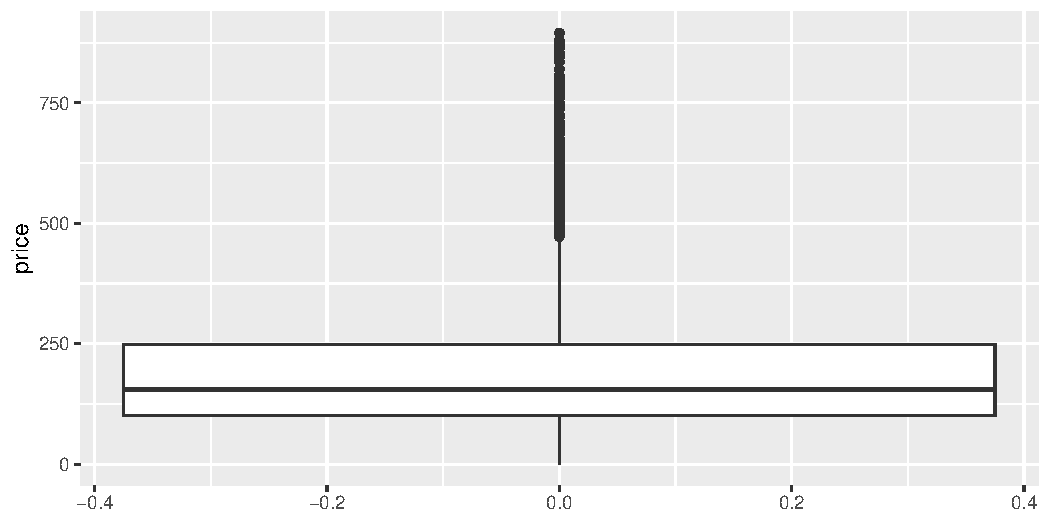
\includegraphics[width=\maxwidth]{figure/chunk-priceBoxPlotLim-1} \end{figure}

\end{knitrout}
Este \textit{boxplot} mostra que a maioria dos alojamentos tem preços entre 103 e 254 USD. Este facto torna-se ainda mais evidente quando analisamos a distribuição dos preços. \\
O gráfico mostra também que há muitos alojamentos fora destes limites, podendo ser valores atípicos também, embora não tão extremos como aqueles vistos anteriormente. No entanto, à primeira vista estes não devem ser valores atípicos, devido à sua quantidade, mesmo quando comparado com o número de registos.\\

\begin{knitrout}
\definecolor{shadecolor}{rgb}{0.969, 0.969, 0.969}\color{fgcolor}\begin{kframe}
\begin{alltt}
\hlkwd{ggplot}\hlstd{(}\hlkwc{data} \hlstd{= df,} \hlkwd{aes}\hlstd{(price))} \hlopt{+} \hlkwd{geom_histogram}\hlstd{(}\hlkwc{binwidth} \hlstd{=} \hlnum{25}\hlstd{,}
    \hlkwd{aes}\hlstd{(}\hlkwc{y} \hlstd{= ..density..))} \hlopt{+} \hlkwd{geom_density}\hlstd{(}\hlkwc{color} \hlstd{=} \hlstr{"red"}\hlstd{)} \hlopt{+}
    \hlkwd{xlim}\hlstd{(}\hlnum{0}\hlstd{, upper_limit)}
\end{alltt}
\end{kframe}\begin{figure}
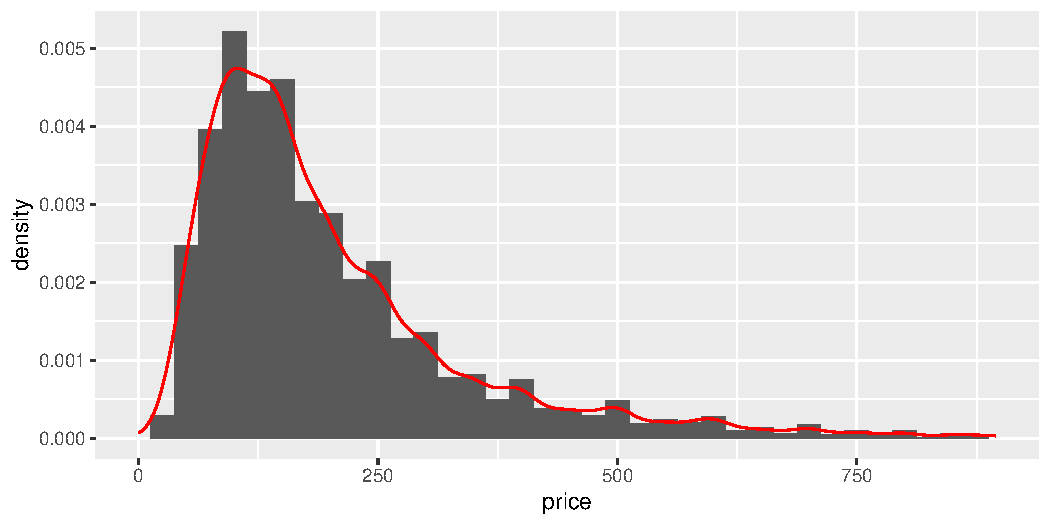
\includegraphics[width=\maxwidth]{figure/chunk-priceHist-1} \end{figure}

\end{knitrout}
A distribuição de preços apresentada demonstra que a maioria dos alojamentos se encontram no limite mostrado anteriormente, e a distribuição parece aproximar-se de uma distribuição $\chi_{k}^{2}$, com um pequeno grau de liberdade. Curiosamente, o gráfico mostra que os preços parecem aumentar algumas vezes a cada 50 USD, o que pode ser devido ao facto de que os hospedeiros escolhem preços redondos, como 50, 100, 175, etc. Este fenómeno parece ser mais visível nos 250 e nos 500.\\

\begin{knitrout}
\definecolor{shadecolor}{rgb}{0.969, 0.969, 0.969}\color{fgcolor}\begin{kframe}
\begin{alltt}
\hlstd{df} \hlopt
    \hlkwd{ggplot}\hlstd{(}\hlkwd{aes}\hlstd{(}\hlkwc{y} \hlstd{= price,} \hlkwc{x} \hlstd{= forcats}\hlopt{::}\hlkwd{fct_reorder}\hlstd{(neighbourhood,}
        \hlstd{price,} \hlkwc{.fun} \hlstd{= median)))} \hlopt{+} \hlkwd{geom_boxplot}\hlstd{()} \hlopt{+}
    \hlkwd{coord_cartesian}\hlstd{(}\hlkwc{ylim} \hlstd{=} \hlkwd{c}\hlstd{(}\hlnum{0}\hlstd{, upper_limit))} \hlopt{+}
    \hlkwd{theme}\hlstd{(}\hlkwc{axis.text.x} \hlstd{=} \hlkwd{element_text}\hlstd{(}\hlkwc{angle} \hlstd{=} \hlnum{90}\hlstd{,}
        \hlkwc{vjust} \hlstd{=} \hlnum{0.5}\hlstd{,} \hlkwc{hjust} \hlstd{=} \hlnum{1}\hlstd{))} \hlopt{+} \hlkwd{labs}\hlstd{(}\hlkwc{x} \hlstd{=} \hlstr{""}\hlstd{)}
\end{alltt}
\end{kframe}\begin{figure}
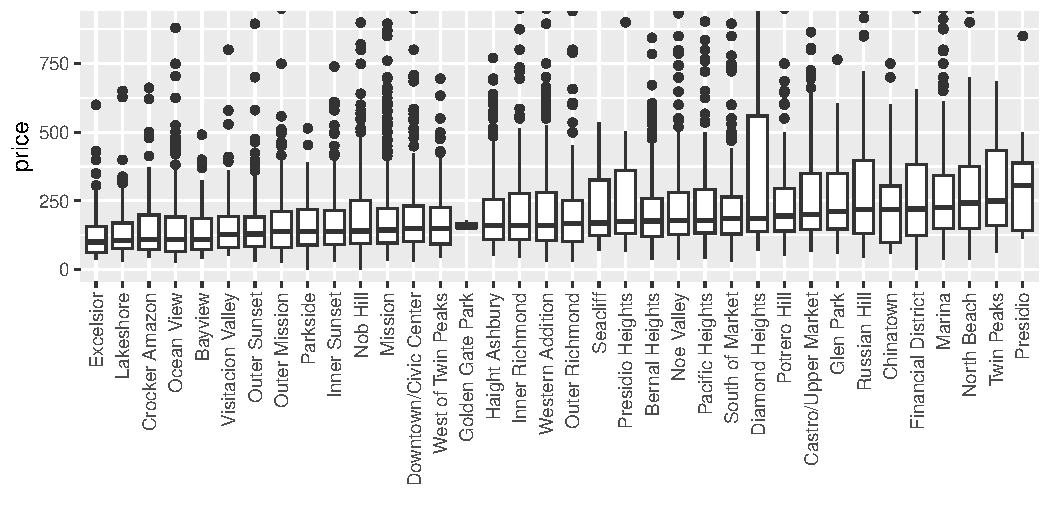
\includegraphics[width=\maxwidth]{figure/chunk-boxPriceNeighs-1} \end{figure}

\end{knitrout}
Os \textit{boxplots} mostram que os preços dos alojamentos não variam bastante de acordo com o bairro sendo que o ponto médio não varia bastante entre bairros, excepto os bairros \textit{Twin Peaks}, e \textit{Presidio}. No entanto, o gráfico mostra uma grande variância dos preços em todos os bairros, exceto no bairro Golden Gate Park.\\

\begin{knitrout}
\definecolor{shadecolor}{rgb}{0.969, 0.969, 0.969}\color{fgcolor}\begin{kframe}
\begin{alltt}
\hlstd{shape_plot} \hlopt{+} \hlkwd{stat_summary_hex}\hlstd{(}\hlkwc{data} \hlstd{= df,}
    \hlkwd{aes}\hlstd{(}\hlkwc{x} \hlstd{= longitude,} \hlkwc{y} \hlstd{= latitude,} \hlkwc{z} \hlstd{=} \hlkwd{log}\hlstd{(price)),}
    \hlkwc{alpha} \hlstd{=} \hlnum{0.8}\hlstd{)} \hlopt{+} \hlkwd{scale_fill_viridis_c}\hlstd{()} \hlopt{+}
    \hlkwd{theme}\hlstd{(}\hlkwc{legend.position} \hlstd{=} \hlstr{"right"}\hlstd{)}
\end{alltt}


{\ttfamily\noindent\color{warningcolor}{\#\# Warning: Removed 3 rows containing non-finite values (`stat\_summary\_hex()`).}}\end{kframe}\begin{figure}
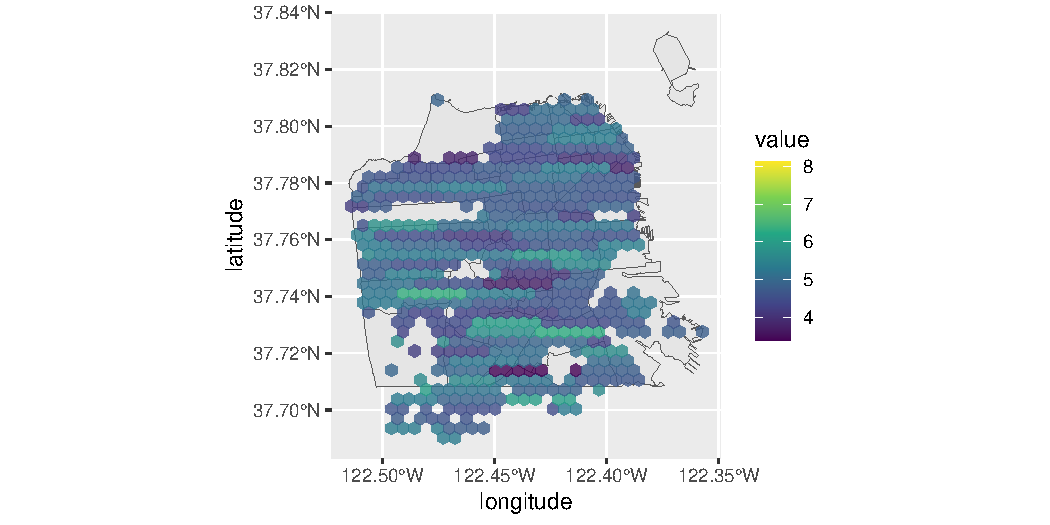
\includegraphics[width=\maxwidth]{figure/chunk-priceHexes-1} \end{figure}

\end{knitrout}

Este gráfico demonstra a variariadade presente nos vários distritos, e da mesma forma não é possível descrever nenhum padrão \textit{a priori} para os preços. \\

\begin{knitrout}
\definecolor{shadecolor}{rgb}{0.969, 0.969, 0.969}\color{fgcolor}\begin{kframe}
\begin{alltt}
\hlstd{df} \hlopt
    \hlkwd{group_by}\hlstd{(room_type)} \hlopt
    \hlkwd{summarise}\hlstd{(}\hlkwc{n} \hlstd{=} \hlkwd{n}\hlstd{(),} \hlkwc{freq} \hlstd{=} \hlkwd{n}\hlstd{()}\hlopt{/}\hlkwd{nrow}\hlstd{(.),}
        \hlkwc{averagePrice} \hlstd{=} \hlkwd{mean}\hlstd{(price),} \hlkwc{sd} \hlstd{=} \hlkwd{sd}\hlstd{(price),}
        \hlkwc{min} \hlstd{=} \hlkwd{min}\hlstd{(price),} \hlkwc{max} \hlstd{=} \hlkwd{max}\hlstd{(price))} \hlopt
    \hlkwd{showT}\hlstd{()}
\end{alltt}
\end{kframe}\begin{table}
\centering\begingroup\fontsize{10}{12}\selectfont

\begin{tabular}{r|r|r|r|r|r|r}
\hline
room\_type & n & freq & averagePrice & sd & min & max\\
\hline
\cellcolor{gray!6}{Entire home/apt} & \cellcolor{gray!6}{4243} & \cellcolor{gray!6}{0.6400664} & \cellcolor{gray!6}{275.8965} & \cellcolor{gray!6}{406.8473} & \cellcolor{gray!6}{33} & \cellcolor{gray!6}{12000}\\
\hline
Hotel room & 65 & 0.0098054 & 266.2154 & 211.0756 & 0 & 1220\\
\hline
\cellcolor{gray!6}{Private room} & \cellcolor{gray!6}{2239} & \cellcolor{gray!6}{0.3377583} & \cellcolor{gray!6}{360.1474} & \cellcolor{gray!6}{1972.6562} & \cellcolor{gray!6}{0} & \cellcolor{gray!6}{25000}\\
\hline
Shared room & 82 & 0.0123699 & 211.7683 & 1101.4410 & 25 & 10000\\
\hline
\end{tabular}
\endgroup{}
\end{table}

\end{knitrout}
A tabela mostra que a maioria dos alojamentos são apartamentos ou casas inteiras, enquanto que os quartos privados são menos frequentes. Mostra também a pequena quantidade de quartos de hotéis e de alojamentos partilhados, sendo estes apenas $2\%$ dos registos. Isto pode levar a que seja necessário o uso de alguma técnica de \textit{oversampling} para os quartos de hotel e para alojamentos partilhados, de forma a aumentar a quantidade de registos destes tipos de alojamentos.\\

A tabela também expõe que os quartos privados são os mais caros em média, enquanto que os alojamentos partilhados são os mais baratos. Esta observação é esperada na parte que diz respeito aos quartos partilhados, no entanto é supreendente que os quartos privados sejam mais caros em média que as casas inteiras e os quartos de hotel. Isto pode ser porque a diferença entre "quarto privado" e "quarto de hotel" pode ser confusa, tanto que os hoteis de alto preço notados em cima estão caracterizados como "quartos privados". Isto pode explicar também o grande desvio padrão das variáveis.\\
\begin{knitrout}
\definecolor{shadecolor}{rgb}{0.969, 0.969, 0.969}\color{fgcolor}\begin{kframe}
\begin{alltt}
\hlstd{df} \hlopt
    \hlkwd{group_by}\hlstd{(room_type)} \hlopt
    \hlkwd{filter}\hlstd{(price} \hlopt{<} \hlstd{upper_limit, price} \hlopt{>} \hlnum{0}\hlstd{)} \hlopt
    \hlkwd{summarise}\hlstd{(}\hlkwc{n} \hlstd{=} \hlkwd{n}\hlstd{(),} \hlkwc{freq} \hlstd{=} \hlkwd{n}\hlstd{()}\hlopt{/}\hlkwd{nrow}\hlstd{(.),}
        \hlkwc{averagePrice} \hlstd{=} \hlkwd{mean}\hlstd{(price),} \hlkwc{sd} \hlstd{=} \hlkwd{sd}\hlstd{(price),}
        \hlkwc{min} \hlstd{=} \hlkwd{min}\hlstd{(price),} \hlkwc{max} \hlstd{=} \hlkwd{max}\hlstd{(price))} \hlopt
    \hlkwd{showT}\hlstd{()}
\end{alltt}
\end{kframe}\begin{table}
\centering\begingroup\fontsize{10}{12}\selectfont

\begin{tabular}{r|r|r|r|r|r|r}
\hline
room\_type & n & freq & averagePrice & sd & min & max\\
\hline
\cellcolor{gray!6}{Entire home/apt} & \cellcolor{gray!6}{4131} & \cellcolor{gray!6}{0.6391769} & \cellcolor{gray!6}{233.9990} & \cellcolor{gray!6}{147.74938} & \cellcolor{gray!6}{33} & \cellcolor{gray!6}{880}\\
\hline
Hotel room & 61 & 0.0094383 & 248.9180 & 151.65776 & 72 & 820\\
\hline
\cellcolor{gray!6}{Private room} & \cellcolor{gray!6}{2191} & \cellcolor{gray!6}{0.3390067} & \cellcolor{gray!6}{135.2793} & \cellcolor{gray!6}{95.85747} & \cellcolor{gray!6}{24} & \cellcolor{gray!6}{800}\\
\hline
Shared room & 80 & 0.0123782 & 78.3125 & 55.54006 & 25 & 300\\
\hline
\end{tabular}
\endgroup{}
\end{table}

\end{knitrout}

Se excluirmos os apartamentos de luxo, conseguimos observar valores mais esperados; quartos de hoteis serem os mais caros com preços aproximados aos das casas inteiras, e os alojamentos partilhados serem os mais baratos. Os preços médios dos quartos privados desceram significativamente. Isto pode ser explicado pela classificação de alojamentos de luxo como "quartos privados". Deste modo suspeitamos que, sem os quartos de luxo, esta nova categoria identifica-se mais com albergues.\\

\begin{knitrout}
\definecolor{shadecolor}{rgb}{0.969, 0.969, 0.969}\color{fgcolor}\begin{kframe}
\begin{alltt}
\hlkwd{ggplot}\hlstd{(df,} \hlkwd{aes}\hlstd{(}\hlkwc{x} \hlstd{= price,} \hlkwc{y} \hlstd{= room_type,}
    \hlkwc{fill} \hlstd{= room_type))} \hlopt{+} \hlkwd{geom_density_ridges}\hlstd{()} \hlopt{+}
    \hlkwd{xlim}\hlstd{(}\hlnum{0}\hlstd{, upper_limit)} \hlopt{+} \hlkwd{theme_ridges}\hlstd{()} \hlopt{+}
    \hlkwd{theme}\hlstd{(}\hlkwc{legend.position} \hlstd{=} \hlstr{"none"}\hlstd{)}
\end{alltt}


{\ttfamily\noindent\itshape\color{messagecolor}{\#\# Picking joint bandwidth of 24.6}}\end{kframe}\begin{figure}
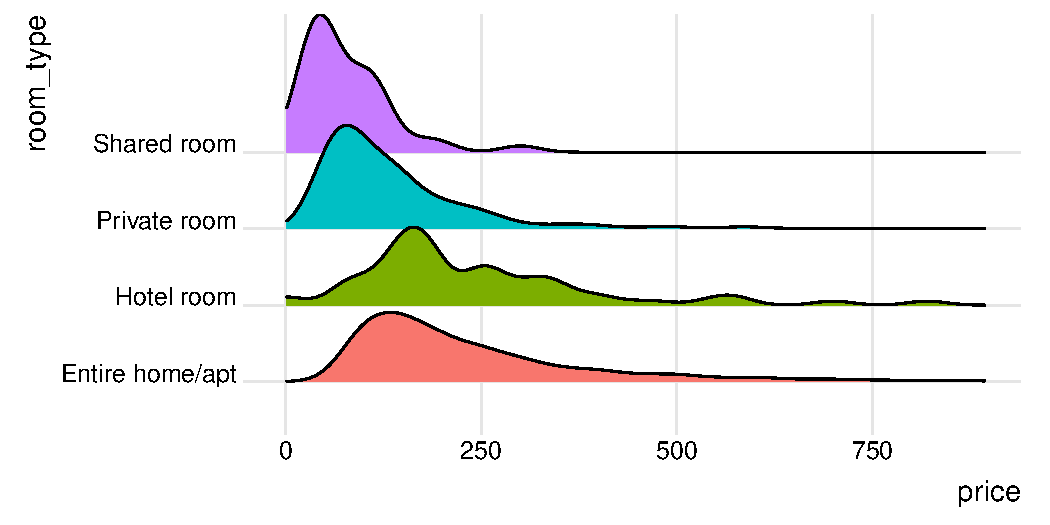
\includegraphics[width=\maxwidth]{figure/chunk-RoomTypesPrice-1} \end{figure}

\end{knitrout}

O diagrama apresentado demonstra as distribuições dos preços por tipo de alojamento. Este corrobora que os quartos de hóteis são os mais caros, mas parece demonstrar também que a maioria dos outros grupos se encontram com preços semelhantes, com uma diferença na densidade na cauda do gráfico, explicando assim a alta média de apartamentos inteiros. desta forma, a maioria dos alojamentos inteiros estão de acordo com quartos privados, mas existem mais alojamentos inteiros mais caros.

\begin{knitrout}
\definecolor{shadecolor}{rgb}{0.969, 0.969, 0.969}\color{fgcolor}\begin{kframe}
\begin{alltt}
\hlstd{df} \hlopt
    \hlkwd{select}\hlstd{(price, latitude, longitude, minimum_nights,}
        \hlstd{number_of_reviews, calculated_host_listings_count,}
        \hlstd{availability_365)} \hlopt
    \hlkwd{cor}\hlstd{(}\hlkwc{use} \hlstd{=} \hlstr{"complete.obs"}\hlstd{)} \hlopt
    \hlkwd{ggcorrplot}\hlstd{(}\hlkwc{lab} \hlstd{=} \hlnum{TRUE}\hlstd{,} \hlkwc{type} \hlstd{=} \hlstr{"lower"}\hlstd{)}
\end{alltt}
\end{kframe}\begin{figure}
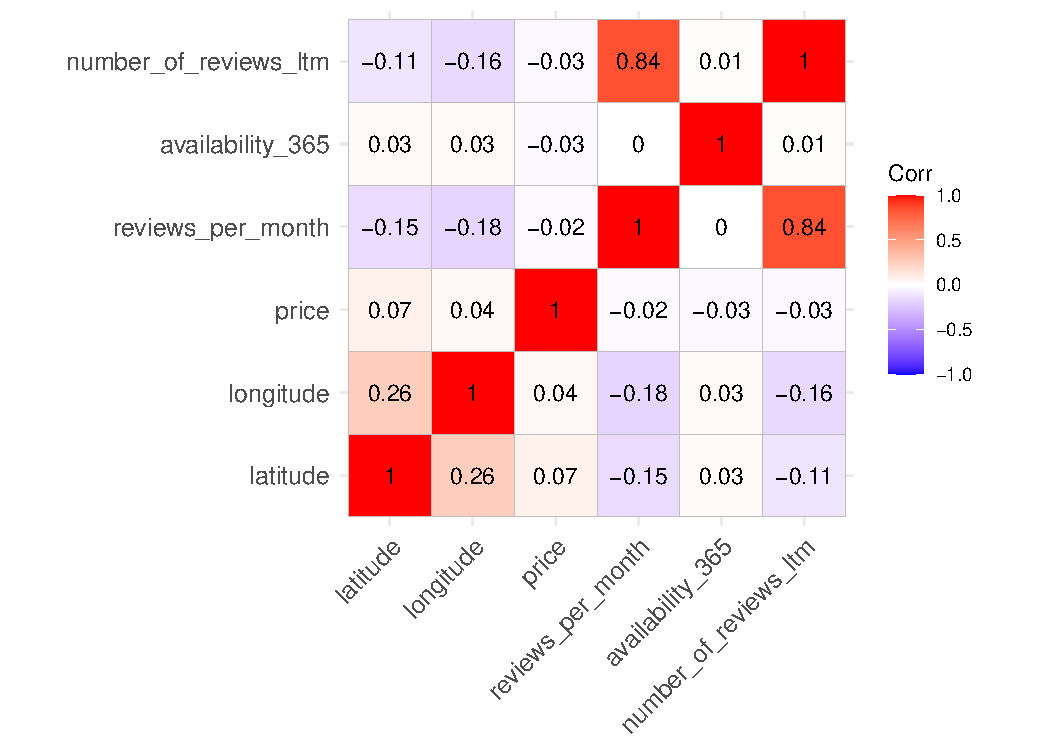
\includegraphics[width=\maxwidth]{figure/chunk-CorrPlot-1} \end{figure}

\end{knitrout}
O gráfico de correlações não mostra também nenhuma correlação significante entre o preço e as outras variáveis numéricas analisaveis. Mostra também uma pouca correlação entre as variáveis independentes.\\


\begin{knitrout}
\definecolor{shadecolor}{rgb}{0.969, 0.969, 0.969}\color{fgcolor}\begin{kframe}
\begin{alltt}
\hlstd{recipeUpSample} \hlkwb{<-} \hlkwd{recipe}\hlstd{(price} \hlopt{~} \hlstd{neighbourhood} \hlopt{+}
    \hlstd{latitude} \hlopt{+} \hlstd{longitude} \hlopt{+} \hlstd{room_type} \hlopt{+} \hlstd{minimum_nights} \hlopt{+}
    \hlstd{number_of_reviews} \hlopt{+} \hlstd{calculated_host_listings_count} \hlopt{+}
    \hlstd{availability_365,} \hlkwc{data} \hlstd{= df)} \hlopt
    \hlkwd{step_upsample}\hlstd{(room_type,} \hlkwc{skip} \hlstd{=} \hlnum{FALSE}\hlstd{,}
        \hlkwc{over_ratio} \hlstd{=} \hlnum{0.363}\hlstd{)} \hlopt
    \hlkwd{step_dummy}\hlstd{(neighbourhood, room_type)} \hlopt
    \hlkwd{prep}\hlstd{()}
\hlstd{recipeNoUpSample} \hlkwb{<-} \hlkwd{recipe}\hlstd{(price} \hlopt{~} \hlstd{neighbourhood} \hlopt{+}
    \hlstd{latitude} \hlopt{+} \hlstd{longitude} \hlopt{+} \hlstd{room_type} \hlopt{+} \hlstd{minimum_nights} \hlopt{+}
    \hlstd{number_of_reviews} \hlopt{+} \hlstd{calculated_host_listings_count} \hlopt{+}
    \hlstd{availability_365,} \hlkwc{data} \hlstd{= df)} \hlopt
    \hlkwd{step_dummy}\hlstd{(neighbourhood, room_type)} \hlopt
    \hlkwd{prep}\hlstd{()}
\hlstd{dfAll} \hlkwb{<-} \hlkwd{bake}\hlstd{(recipeUpSample, df} \hlopt
    \hlkwd{filter}\hlstd{(price} \hlopt{>} \hlnum{0}\hlstd{))}
\hlstd{dfAll} \hlopt
    \hlkwd{group_by}\hlstd{(}\hlkwc{isHotel} \hlstd{= room_type_Hotel.room,}
        \hlkwc{isPrivateRoom} \hlstd{= room_type_Private.room,}
        \hlkwc{isSharedRoom} \hlstd{= room_type_Shared.room)} \hlopt
    \hlkwd{summarise}\hlstd{(}\hlkwc{n} \hlstd{=} \hlkwd{n}\hlstd{(),} \hlkwc{freq} \hlstd{= n}\hlopt{/}\hlkwd{nrow}\hlstd{(dfAll),}
        \hlkwc{averagePrice} \hlstd{=} \hlkwd{mean}\hlstd{(price))} \hlopt
    \hlkwd{showT}\hlstd{()}
\end{alltt}
\end{kframe}\begin{table}
\centering\begingroup\fontsize{10}{12}\selectfont

\begin{tabular}{r|r|r|r|r|r}
\hline
isHotel & isPrivateRoom & isSharedRoom & n & freq & averagePrice\\
\hline
\cellcolor{gray!6}{0} & \cellcolor{gray!6}{0} & \cellcolor{gray!6}{0} & \cellcolor{gray!6}{4243} & \cellcolor{gray!6}{0.4437820} & \cellcolor{gray!6}{271.0295}\\
\hline
0 & 0 & 1 & 1540 & 0.1610710 & 212.9039\\
\hline
\cellcolor{gray!6}{0} & \cellcolor{gray!6}{1} & \cellcolor{gray!6}{0} & \cellcolor{gray!6}{2238} & \cellcolor{gray!6}{0.2340759} & \cellcolor{gray!6}{391.4486}\\
\hline
1 & 0 & 0 & 1540 & 0.1610710 & 274.1903\\
\hline
\end{tabular}
\endgroup{}
\end{table}

\end{knitrout}
A quantidade de hotéis e alojoamentos partilhados foram aumentada para 1540 (ainda inclui desequilíbrio, mas devido à realmente pequena quantidade destes decidimos não equilibrar demasiado), e as nossas variáveis categóricas foram transformadas em \textit{dummies}, de forma a tornar possível a sua análise.\\

Para analisar e comparar modelos, vai ser usado \textit{in-sample} e analisado as estatísticas do coeficiente de determinação $R^2$, e o \textit{MAPE}. A estatística $F$ vai ser insignificante pare o nosso modelo, devido à grande quantidade de observações, levando a uma rejeição da hipótese nula constante. Para comparar modelos, vai ser observado o \textit{AIC} de cada, quando apropriado. Para verificar os pressupostos, vai ser analisado se a média dos resíduos padrozinados é praticamente zero, o teste de \textit{Breusch-Pagan} para verificar a homocedasticidade, o teste de \textit{Breusch-Godfrey} para verificar a autocorrelação, e o teste de \textit{Jarque-Bera} para verificar a normalidade dos resíduos. Em alguns modelos vai ser também analisado o gráficos de resíduos.\\

Em cada um destes testes, se o valor $p$ for menor que $0.05$, então rejeitamos $H_0$. No teste \textit{Breusch-Pagan}, $H_0$ é que os resíduos são homocedásticos, e no teste \textit{Breusch-Godfrey}, $H_0$ é que os resíduos não são autocorrelacionados. No teste \textit{Jarque-Bera}, $H_0$ é que os resíduos são normais.\\

O nosso primeiro modelo linear foi um modelo que diretamente relaciona as variáveis todas com o preço. \\
\begin{knitrout}
\definecolor{shadecolor}{rgb}{0.969, 0.969, 0.969}\color{fgcolor}\begin{kframe}
\begin{alltt}
\hlstd{fit0} \hlkwb{<-} \hlkwd{lm}\hlstd{(price} \hlopt{~} \hlstd{., dfAll)}
\hlstd{fit0} \hlopt
    \hlkwd{glance}\hlstd{()} \hlopt
    \hlkwd{select}\hlstd{(}\hlkwc{R2} \hlstd{= r.squared,} \hlkwc{AIC} \hlstd{= AIC)} \hlopt
    \hlkwd{mutate}\hlstd{(}\hlkwc{MAPE} \hlstd{=} \hlkwd{MAPE}\hlstd{(dfAll}\hlopt{$}\hlstd{price,} \hlkwd{predict}\hlstd{(fit0,}
        \hlstd{dfAll)),} \hlkwc{`Breusch-Pagan`} \hlstd{=} \hlkwd{validP}\hlstd{(}\hlkwd{bptest}\hlstd{(fit0)}\hlopt{$}\hlstd{p.value,}
        \hlnum{FALSE}\hlstd{),} \hlkwc{`Breusch-Godfrey`} \hlstd{=} \hlkwd{validP}\hlstd{(}\hlkwd{bgtest}\hlstd{(fit0)}\hlopt{$}\hlstd{p.value,}
        \hlnum{FALSE}\hlstd{),} \hlkwc{`Jarque-Bera`} \hlstd{=} \hlkwd{validP}\hlstd{(}\hlkwd{jarque.bera.test}\hlstd{(fit0}\hlopt{$}\hlstd{residuals)}\hlopt{$}\hlstd{p.value,}
        \hlnum{TRUE}\hlstd{))} \hlopt
    \hlkwd{t}\hlstd{()} \hlopt
    \hlkwd{showT}\hlstd{()}
\end{alltt}
\end{kframe}\begin{table}
\centering\begingroup\fontsize{10}{12}\selectfont

\begin{tabular}{l|r}
\hline
R2 & 0.04582814\\
\hline
\cellcolor{gray!6}{AIC} & \cellcolor{gray!6}{161374.8}\\
\hline
MAPE & 3.782943\\
\hline
\cellcolor{gray!6}{Breusch-Pagan} & \cellcolor{gray!6}{p = 1.57675882618306e-50}\\
\hline
Breusch-Godfrey & p > 0.05\\
\hline
\cellcolor{gray!6}{Jarque-Bera} & \cellcolor{gray!6}{p < 0.05}\\
\hline
\end{tabular}
\endgroup{}
\end{table}

\begin{kframe}\begin{alltt}
\hlkwd{plot}\hlstd{(fit0,} \hlnum{1}\hlstd{)}
\end{alltt}
\end{kframe}\begin{figure}
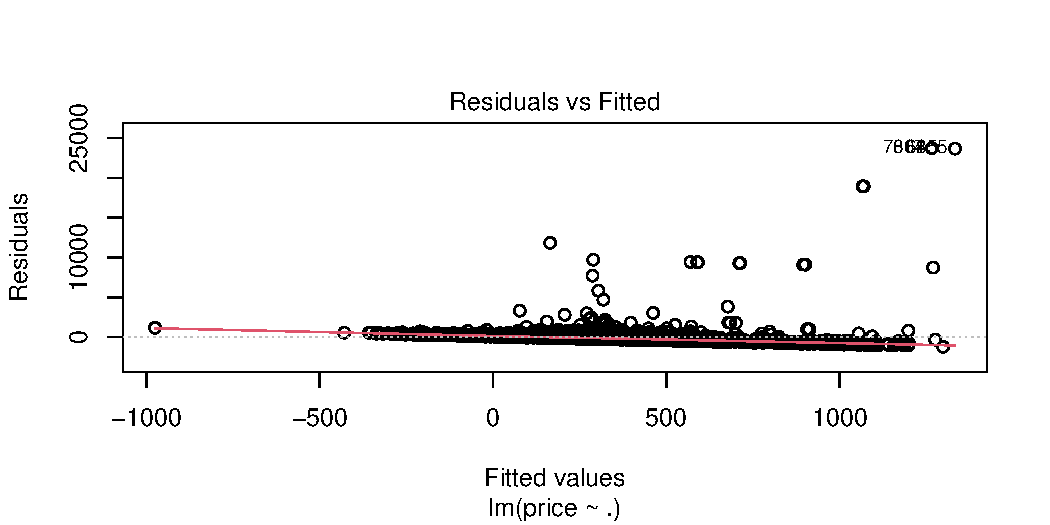
\includegraphics[width=\maxwidth]{figure/chunk-fit0-1} \end{figure}

\end{knitrout}



\bibliography{references}{}
\bibliographystyle{plain}
\end{document}
